\section{Discussion}
\label{sec:discussion}

\subsection{Task-dependent effects of linguistic partitioning}

The ablation results show that the usefulness of a representation depends
strongly on the downstream task. No language-modeling method was uniformly
best across Analogy, Morphology, named entity recognition (NER),
part-of-speech tagging (POS), and Sentiment classification. This pattern
argues against selecting a single segmentation strategy solely from its
aggregate performance. Instead, the appropriate representation appears to
depend on whether the task primarily requires lexical-semantic information,
morphological structure, or sequence-level label discrimination.

The unpartitioned \texttt{lm-word} condition provides an informative baseline
for this interpretation. It performed poorly on Analogy
(Accuracy $=0.000143$), NER ($F_1=0.126547$), and POS
($F_1=0.026706$), while matching \texttt{frequent-ngram} on Morphology
($F_1=0.345762$). In contrast, it was competitive on Sentiment
(Accuracy $=0.828200$, $F_1=0.651535$). The contrast suggests that lexical
identity can be sufficient for document-level polarity classification, but
that unpartitioned word representations are less effective for tasks that
depend on productive word structure or token-level contextual distinctions.
Because \texttt{lm-word} was represented by only one configuration per task,
these values should be interpreted as baseline observations rather than
estimates of its expected performance or stability.

\subsection{Analogy and Morphology}

For Analogy, \texttt{lm-subword} produced the highest observed Accuracy
($0.037762$), followed by the best \texttt{lm-lemma} configuration
($0.032602$). The method-level distribution nevertheless indicates that
\texttt{lm-lemma} was more stable near the upper end of the observed range,
whereas \texttt{lm-subword} achieved a higher peak with greater variation
across configurations. This distinction is important for model selection:
subword modeling offered the strongest tuned result, while lemma-based
modeling offered more consistent performance under the evaluated
hyperparameter settings. All Analogy scores were low in absolute terms, so
the results support only a relative comparison among representations; they do
not indicate strong absolute relational reasoning. The legacy
\texttt{F1-MEASURE} field associated with Analogy is an unbounded similarity
output and was therefore excluded from comparison.

Morphology exhibited a related trade-off between peak performance and
robustness. The best \texttt{lm-skip} variant reached $F_1=0.538576$, which
was the highest observed Morphology F-measure. The best \texttt{lm-rank}
variant reached $0.493722$, and \texttt{lm-lemma} reached $0.475877$.
However, every evaluated \texttt{lm-lemma} configuration produced the same
reported F-measure, whereas \texttt{lm-skip} varied substantially across its
grid. Thus, \texttt{lm-skip} is preferable if the objective is the highest
attained score and tuning is available, while \texttt{lm-lemma} is the more
conservative choice when robustness to the tested settings is important.
The much lower word-level baseline reinforces the conclusion that explicit
linguistic or sublexical structure is beneficial for morphological
generalization.

\subsection{Sequence-labeling tasks}

The current, fully measured NER results favored representations that expose
linguistically meaningful internal structure. The strongest comparable
F-measure was obtained by \texttt{lm-syllable} ($0.682859$), followed by
\texttt{lm-skip} ($0.669862$) and the best current \texttt{lm-lemma}
configuration ($0.660480$). By comparison, \texttt{lm-word} obtained only
$0.126547$. The large difference between the word baseline and the structured
representations is consistent with NER benefiting from recurring form-based
signals that generalize beyond individual word types. At the same time, the
relatively high token Accuracy values and lower macro-F-measures demonstrate
that Accuracy alone can obscure performance on less frequent entity classes.
Consequently, the NER interpretation should prioritize the current
class-balanced F-measure.

POS displayed a similar pattern. The best current result was obtained by
\texttt{lm-lemma} ($F_1=0.645612$), closely followed by
\texttt{lm-subword} ($0.642950$), \texttt{lm-syllable} ($0.633460$), and
\texttt{lm-rank} ($0.625917$). The \texttt{frequent-ngram} baseline was lower
($0.481695$), and \texttt{lm-word} was substantially lower
($0.026706$). The small separation among the leading structured methods
suggests that several forms of linguistic decomposition can capture useful
grammatical regularities. The present design does not establish that the
numerically best method is reliably superior, but it clearly separates the
leading structured representations from the unpartitioned word baseline.

Nine historical artifacts report an F-measure without Precision or Recall:
all are \texttt{lm-skip} POS rows. These values predate the current
macro-F-measure implementation and include unusually high scores. They were
retained for traceability but were excluded from comparative figures, method
means, hyperparameter sensitivity estimates, and selection of the best
current POS configurations. All 96 NER variants now contain complete
Accuracy, Precision, Recall, and F-measure fields.

\subsection{Sentiment classification}

Sentiment differed from the token-level tasks. The best observed F-measure was
produced by \texttt{lm-skip} ($0.678592$), followed by
\texttt{lm-subword} ($0.669665$), \texttt{lm-syllable} ($0.661312$), and
\texttt{lm-word} ($0.651535$). The word baseline therefore remained within
the leading range, despite its poor NER and POS performance. This result is
consistent with Sentiment depending more directly on lexical polarity and
sentence-level semantic composition than on fine-grained token categories.
Structured partitioning still improved the best observed score, but its
advantage was smaller than in the sequence-labeling tasks. The best Sentiment
Accuracy and F-measure were also obtained by different configurations, which
shows that model selection can change with the evaluation criterion.

\subsection{Hyperparameter definitions and experimental scope}

Table~\ref{tab:hyperparameters} defines the LM hyperparameters reported in the
ablation tables. The parameters control three related stages: construction of
the local context, generation of candidate token partitions, and scoring or
regularization of the induced graph. Their interpretation is
method-dependent because not every LM implementation consumes every
parameter.

\begin{table*}[t]
  \centering
  \small
  \begin{tabular}{
    p{0.18\textwidth}
    p{0.12\textwidth}
    p{0.27\textwidth}
    p{0.28\textwidth}
  }
    \hline
    Parameter & Evaluated values & Operational definition &
    Interpretation \\
    \hline
    \texttt{lmWindowLength} ($W$)
    & $2,3,4$
    & Number of consecutive input tokens considered when training or
      selecting a locally coherent partition sequence.
    & Larger values provide broader contextual evidence but enlarge the
      candidate-combination space. The \texttt{lm-word} baseline retains its
      default value of $10$, although it performs no subword partitioning.
      \\

    \texttt{lmSlideLength} ($S$)
    & $2,3,4$
    & Number of partition units in the local sequence window accumulated by
      the transducer. Successive windows advance by one position.
    & Controls the order of the local sequential statistics; despite its
      name, it is a window length rather than the stride between windows.
      \\

    \texttt{lmTopSplit} ($K$)
    & $1,3,5$
    & Maximum number of candidate segmentations retained for each token
      before sentence-level combinations are scored.
    & Larger values increase candidate diversity and computational cost,
      whereas smaller values impose a more selective partition search.
      \\

    \texttt{lmSkip} ($D$)
    & $2,3,4$
    & Maximum backward distance used when adding or scoring skip
      dependencies between partition units.
    & Determines the contextual horizon of non-adjacent graph connections;
      larger values permit longer-range dependencies.
      \\

    \texttt{lmStemLength} ($L_{\min}$)
    & $7$
    & Minimum prefix length from which stem--remainder candidates are
      generated during dictionary construction.
    & Restricts very short stem candidates. Tokens no longer than this
      threshold remain available as unsplit whole-token candidates.
      \\

    \texttt{lmPrune} ($P$)
    & $100$
    & Maximum number of high-scoring outgoing transitions retained at each
      transducer or rank state when pruning is enabled.
    & Bounds graph branching and memory use while preserving the strongest
      observed transitions.
      \\

    \texttt{lmLikelihoodWeight} ($\lambda_{\mathrm{like}}$)
    & $0,.05,.15,$\newline $.30,.50$
    & Weight assigned to contextual transition likelihood in the
      \texttt{RankLM} score update.
    & Larger values increase the contribution of graph-based contextual
      evidence relative to the candidate's existing score.
      \\

    \texttt{lmPriorWeight} ($\lambda_{\mathrm{prior}}$)
    & $1,.95,.85,$\newline $.70,.50$
    & Weight assigned to the current or prior candidate score in
      \texttt{RankLM}.
    & Preserves evidence already associated with a candidate. In the
      evaluated grid,
      $\lambda_{\mathrm{prior}}=1-\lambda_{\mathrm{like}}$.
      \\

    \texttt{lmLengthPenalty}
    & none; inverse parts; inverse square-root parts; inverse log parts
    & Rescales a candidate score $s$ according to its number of non-empty
      partitions $m$.
    & Controls the influence of segmentation granularity on ranking, with
      progressively different normalization rates for multi-part candidates.
      \\
    \hline
  \end{tabular}
  \caption{Operational definitions of the LM hyperparameters used in the
  ablation experiments.}
  \label{tab:hyperparameters}
\end{table*}

For \texttt{RankLM}, the contextual update can be summarized as
\begin{equation}
  s_i^{\prime}
  =
  \lambda_{\mathrm{prior}}s_i
  +
  \lambda_{\mathrm{like}}\ell_i,
\end{equation}
where $s_i$ is the current candidate score and $\ell_i$ is its estimated
forward-transition likelihood. The tested length normalizations take the
form
\begin{equation}
  \widetilde{s}
  =
  \frac{s}{g(m)},
  \qquad
  g(m)\in
  \left\{
    1,\,
    m,\,
    \sqrt{m},\,
    \log(m+1)
  \right\}.
\end{equation}
The four choices correspond respectively to no penalty, inverse-parts,
inverse-square-root-parts, and inverse-log-parts normalization.

The supplementary \texttt{lm-subword} configurations also vary
\texttt{lmSample} over $5$, $10$, and $20$. This parameter limits the number
of entropy-ranked token partitions sampled after applying
\texttt{lmTopSplit}; its effective value is consequently bounded by the
number of retained candidates. The ranking iteration count is fixed at $10$
and is not part of the ablation grid.

Several design constraints limit one-parameter interpretation. In the base
grid, $W$, $S$, and $D$ are assigned the same value and therefore vary
together. Likewise, the likelihood and prior weights are complementary rather
than independently manipulated. Moreover, the likelihood/prior weighting and
length normalization are directly implemented by \texttt{RankLM};
\texttt{LemmaLM} records these settings for grid symmetry but does not
directly reference them in its current scoring path. Finally,
\texttt{lmStemLength} and \texttt{lmPrune} remain fixed at $7$ and $100$,
respectively, and their individual effects cannot be estimated from this
experiment.

\subsection{Hyperparameter sensitivity}

The sensitivity analysis used Analogy Accuracy and F-measure for all other
tasks, matching the metrics used in the distribution comparisons.
\texttt{lm-top-split} had the largest median descriptive effect for every
selected task metric: Analogy Accuracy ($0.83$), Morphology F-measure
($0.83$), NER F-measure ($0.51$), POS F-measure ($0.53$), and Sentiment
F-measure ($0.56$). This recurring pattern suggests that the number of
retained candidate splits is an important practical control on representation
quality. For NER, the complementary likelihood and prior weights were the
next-largest effects ($0.33$ each), followed by the coupled window, slide, and
skip parameters ($0.27$ each). Sentiment also showed a secondary association
with length penalty ($0.30$).

These sensitivity values are descriptive rather than causal. Window length,
slide length, and skip length co-vary in much of the design, while likelihood
and prior weights are complementary. Their apparent effects therefore cannot
be interpreted as independent contributions. In addition, unequal method
grids and legacy sequence-labeling artifacts can influence grouped means.
The sensitivity results are most appropriately used to prioritize a smaller,
balanced confirmatory grid rather than to make mechanistic claims.

\begin{table*}[t]
  \centering
  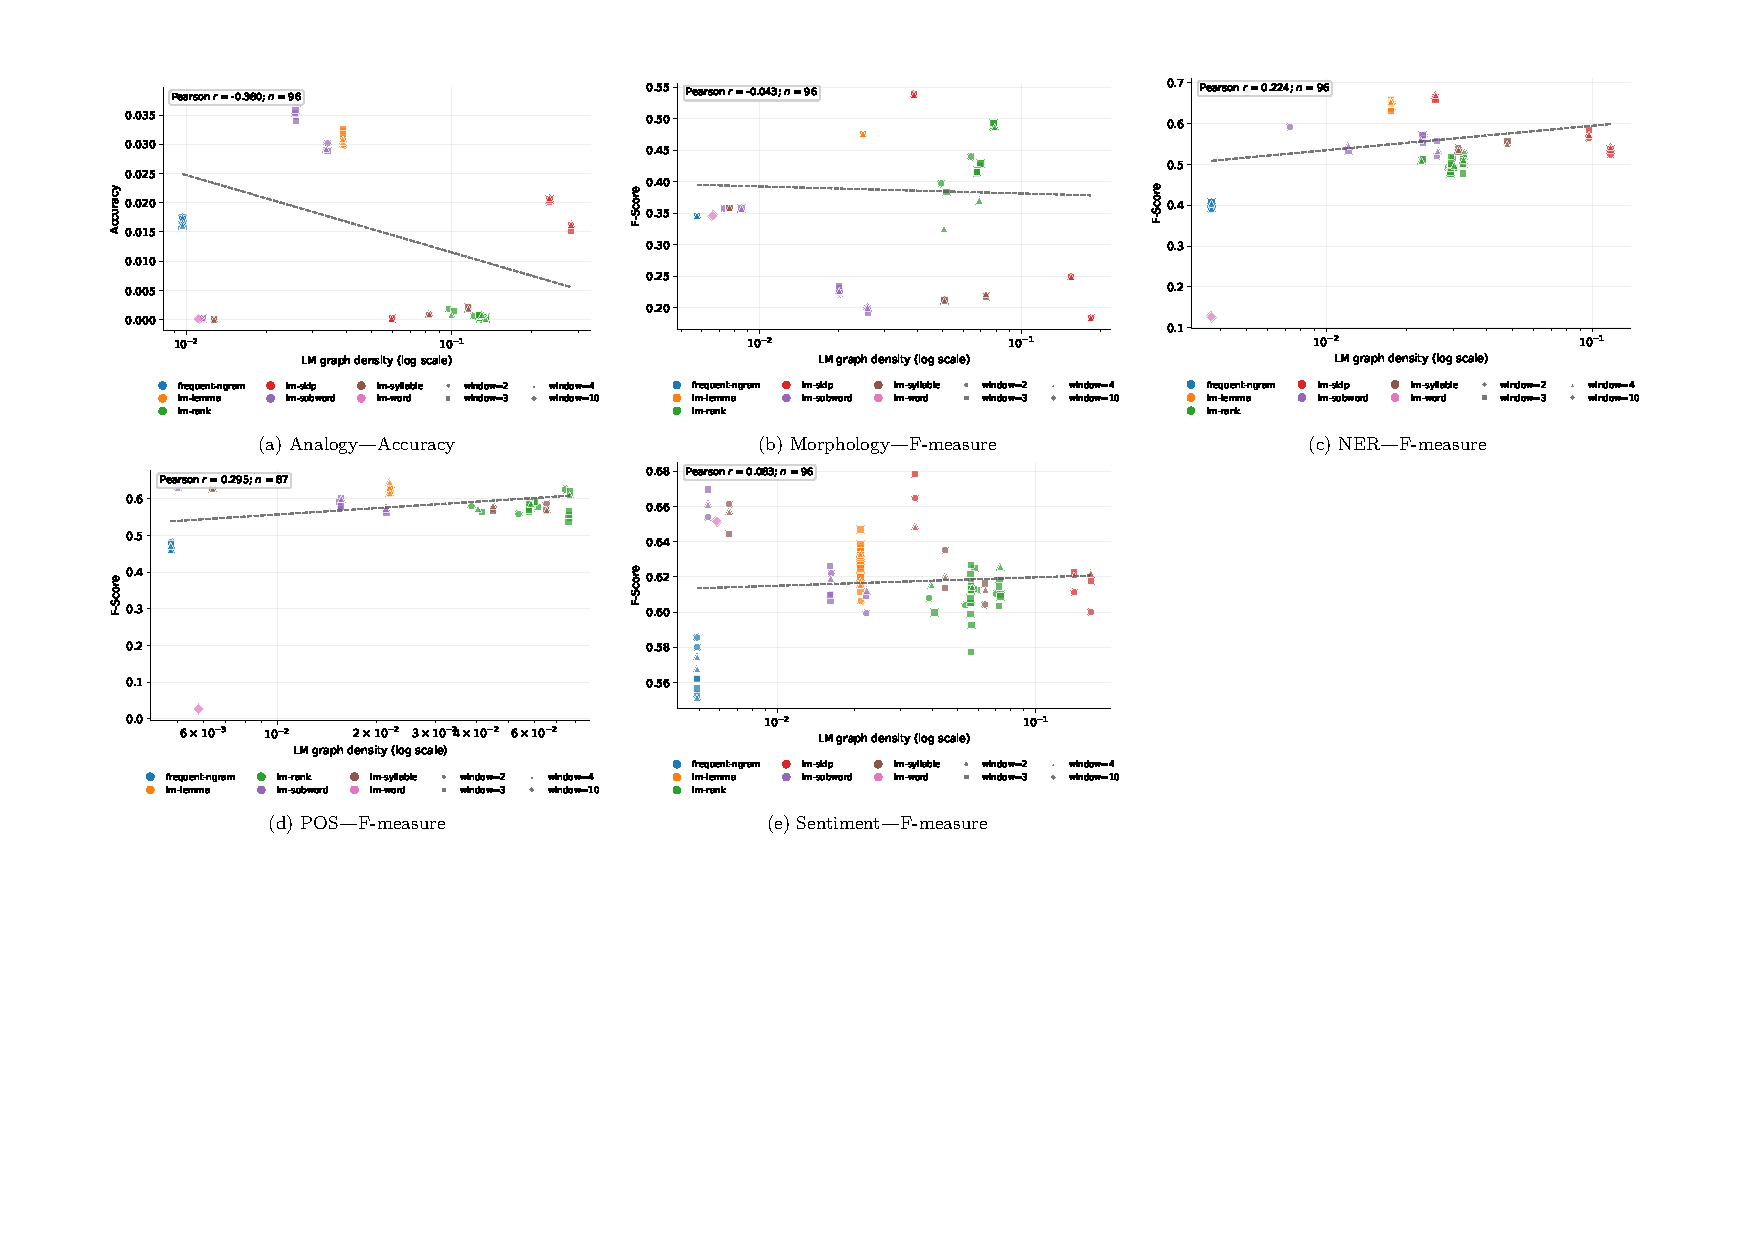
\includegraphics[
    width=\textwidth,
    keepaspectratio
  ]{plots/lm_graph_density_3x2_table.pdf}
  \caption{Relationship between LM graph density and task performance.
  Density is shown on a logarithmic scale. Analogy is evaluated with
  Accuracy, while Morphology, NER, POS, and Sentiment are evaluated with
  F-measure.}
  \label{tab:density}
\end{table*}

\subsection{LM graph density and task performance}

Table~\ref{tab:density} relates the density of the graph induced by each
partitioned corpus to downstream performance. Following the implementation in
\texttt{LMDataset}, graph density is calculated as
$D=2E/[V(V-1)]$, where $E$ is the total weight of the ordered within-sentence
connections between LM partitions and $V$ is the number of distinct
partitions in a deterministic sample of at most 10,000 non-empty sentences.
Thus, denser graphs indicate that the observed partition vocabulary is
connected more frequently within sentences \citep{west2001}. Density is shown
on a logarithmic scale because its empirical range spans more than one order
of magnitude. The task metric follows the rest of the analysis: Accuracy is
used for Analogy, whereas F-measure is used for Morphology, NER, POS, and
Sentiment.

The results do not support a uniform relationship between graph density and
task performance. The descriptive Pearson correlations between log-density
and task score are approximately null for Morphology ($r=-0.043$) and
Sentiment ($r=0.083$). NER ($r=0.224$) and POS ($r=0.295$) show weak positive
associations, whereas Analogy shows a moderate negative association between
log-density and Accuracy ($r=-0.380$). The Morphology value uses the mean
density of the same LM variant across the four stored partition corpora
because the direct Morphology evaluation does not save a partitioned corpus.
The differing directions and magnitudes indicate that neither uniformly
dense nor uniformly sparse representations can be preferred across tasks.

These correlations are descriptive and should not be interpreted as
independent effects of density. LM method, window size, and the remaining
partition parameters jointly determine both the graph structure and the
resulting representation, so the scatter plots combine between-method and
within-method variation. The results therefore suggest that graph density
alone is insufficient for model selection; the identity and linguistic
quality of the retained partitions remain important. A confirmatory analysis
would vary density while holding the partition method and tuning budget
fixed, and would construct and save a task-specific partition corpus for
Morphology.

\begin{table*}[t]
  \centering
  \begin{tabular}{@{}ccc@{}}
    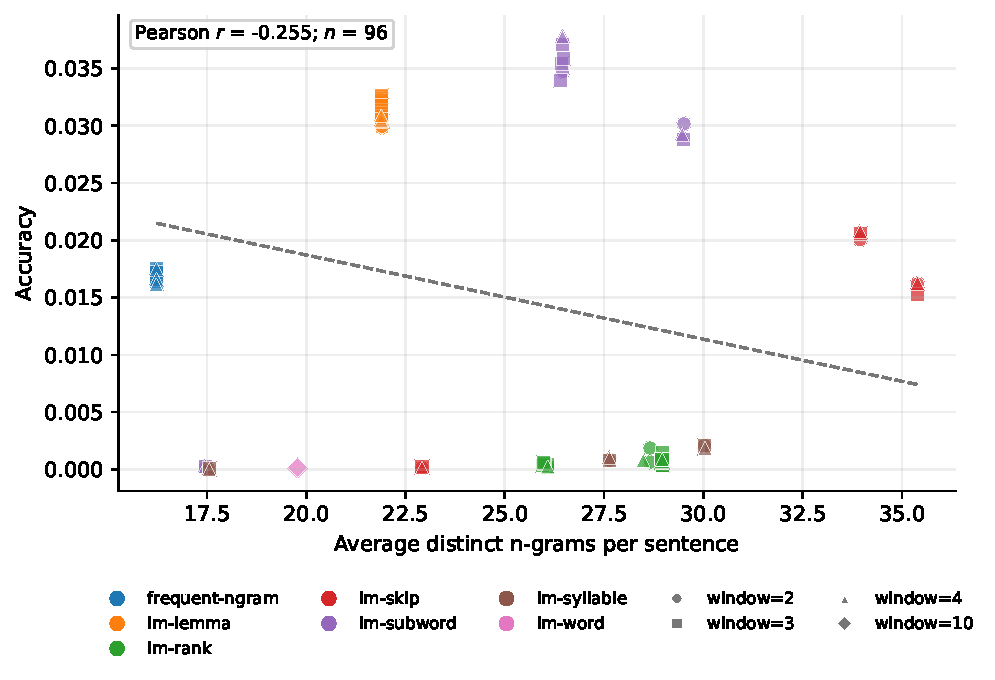
\includegraphics[
      width=0.315\textwidth,
      keepaspectratio
    ]{plots/avg-intrinsic.pdf}
    &
    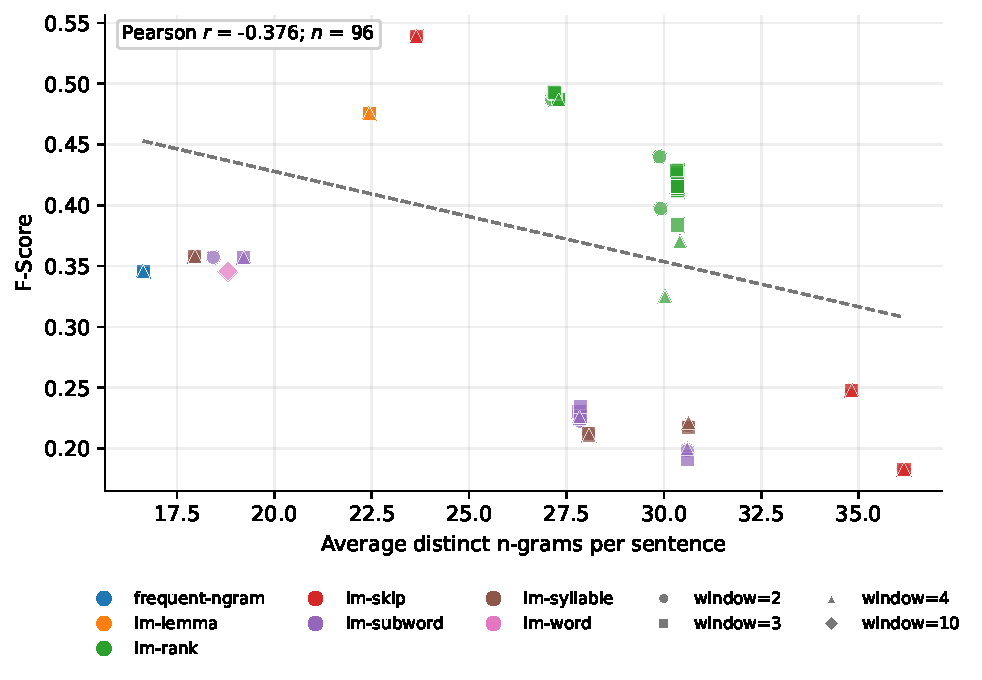
\includegraphics[
      width=0.315\textwidth,
      keepaspectratio
    ]{plots/avg-morphology.pdf}
    &
    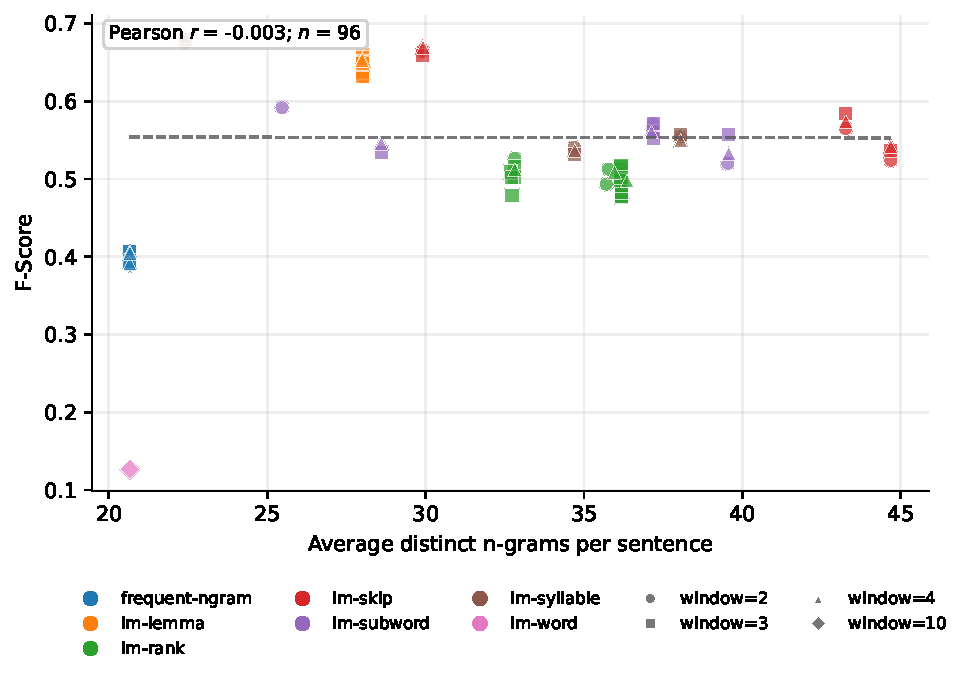
\includegraphics[
      width=0.315\textwidth,
      keepaspectratio
    ]{plots/avg-ner.pdf}
    \\
    Intrinsic & Morphology & NER
    \\
    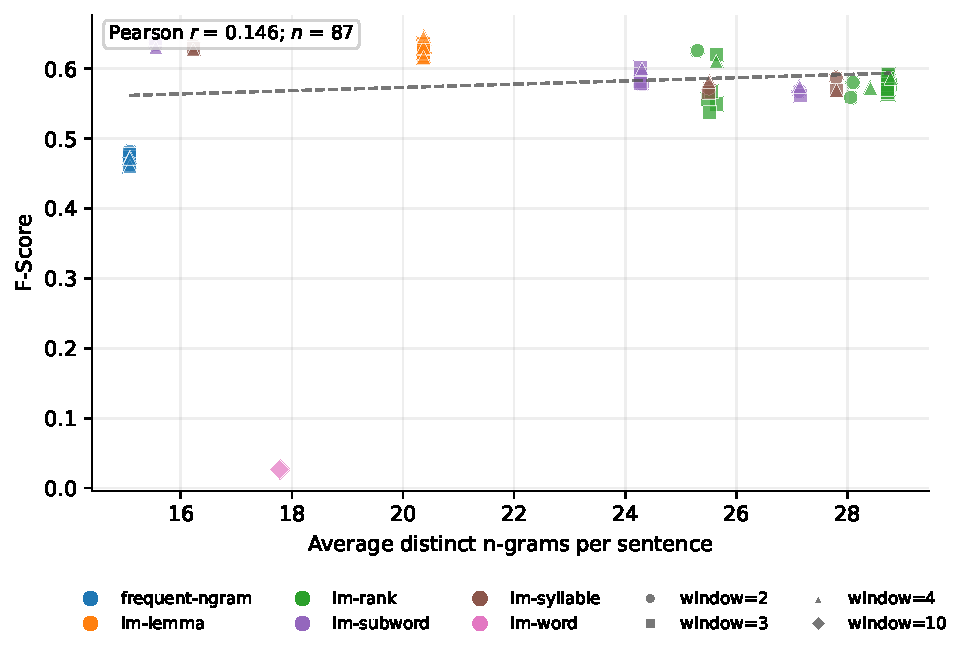
\includegraphics[
      width=0.315\textwidth,
      keepaspectratio
    ]{plots/avg-pos.pdf}
    &
    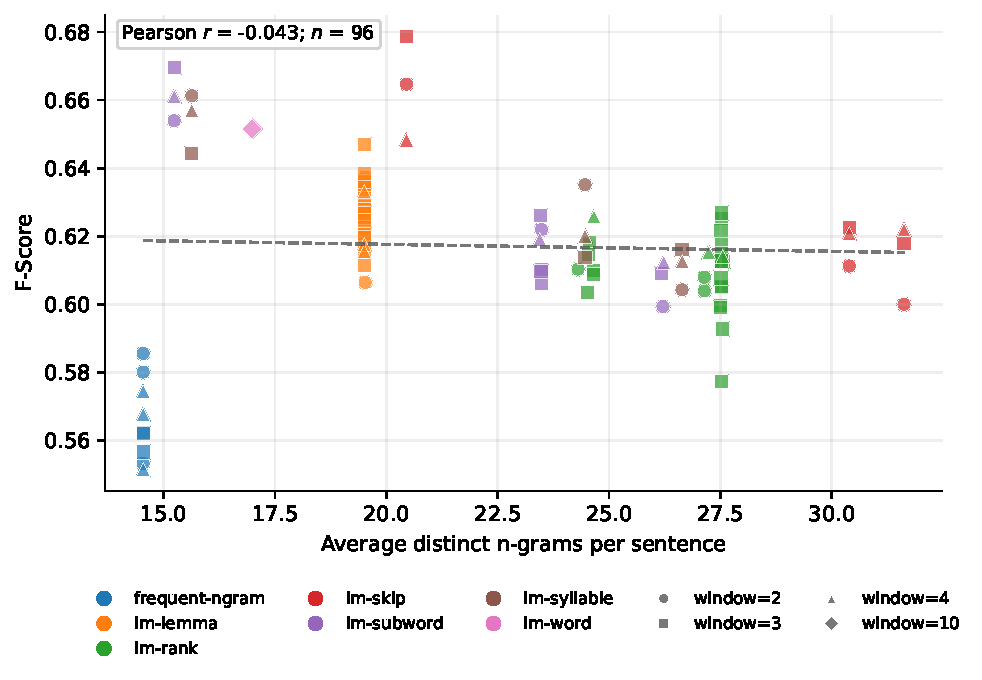
\includegraphics[
      width=0.315\textwidth,
      keepaspectratio
    ]{plots/avg-sentiment.pdf}
    &
    {}
    \\
    POS & Sentiment & {}
  \end{tabular}
  \caption{Average number of distinct LM n-grams per sentence and task
  performance. Intrinsic uses Accuracy; Morphology, NER, POS, and Sentiment
  use F-measure.}
  \label{tab:avg}
\end{table*}

\subsection{Distinct n-gram diversity and task performance}

Table~\ref{tab:avg} examines whether the average number of distinct LM
n-grams in a sentence is associated with downstream performance. For each
stored partition corpus, the number of unique partitions is first calculated
within every sampled sentence and then averaged over at most 10,000 non-empty
sentences. This statistic measures local representational diversity: larger
values indicate that a typical sentence contains a wider variety of
partition units. Intrinsic performance is represented by Accuracy, while
Morphology, NER, POS, and Sentiment are represented by F-measure.

No consistent relationship emerges across tasks. The descriptive Pearson
correlation is negative for Intrinsic Accuracy ($r=-0.255$) and the
Morphology reference estimate ($r=-0.376$). NER ($r=-0.003$) and Sentiment
($r=-0.043$) are approximately uncorrelated with distinct-n-gram diversity,
whereas POS shows a weak positive association ($r=0.146$). Thus, increasing
the number of distinct partitions in a sentence does not uniformly improve
or degrade performance. The result suggests that the linguistic relevance
and selection of the partitions are more consequential than their quantity
alone.

As in the density analysis, these correlations combine variation in LM
method, window length, and other partition parameters and therefore do not
identify an independent causal effect. All NER rows are current; the POS panel
excludes the nine legacy rows without Precision and Recall. Morphology
requires an additional limitation: its direct evaluator does not save a
partitioned corpus, so its x-axis value is the mean distinct-n-gram count of
the same LM variant across the four stored partition corpora. A future
evaluation should save the Morphology partitions and repeat the analysis
using a directly measured, task-specific value.

\subsection{Implications, limitations, and future evaluation}

Taken together, the experiments indicate that linguistic partitioning is most
valuable when a task requires generalization across word forms or
token-level grammatical and entity categories. Lemma, syllable, skip, rank,
and subword representations each provided an advantage for at least one such
objective. The competitive \texttt{lm-word} Sentiment result further shows
that additional segmentation complexity is not uniformly necessary.
Accordingly, task-specific selection is better supported than a universal
ranking of representation methods.

The conclusions remain subject to several limitations. First, the study uses
fixed train/test splits and reports no repeated-run uncertainty or
significance tests; numerical differences must therefore be described as
observed rather than statistically significant. Second, the methods were
evaluated with unequal numbers of variants: one for \texttt{lm-word} and
9, 12, or 28 for the other methods. Methods with larger search spaces have
more opportunities to produce an extreme maximum, making peak comparisons
optimistic. Third, the nine legacy \texttt{lm-skip} POS results are not fully
comparable with outputs from the current evaluator and are retained only for
traceability. Finally, several parameters were varied jointly, limiting the
interpretability of one-factor sensitivity summaries.

A confirmatory study should rerun all selected configurations with the same
metric implementation, use repeated random seeds, and allocate an equal tuning
budget to each method. The strongest configurations should then be evaluated
on an untouched test set or through a repeated validation protocol. Such a
design would permit uncertainty intervals and formal comparisons while
preserving the task-specific metric policy used here: Accuracy for Analogy and
F-measure for Morphology, with macro-F-measure for NER, POS, and Sentiment.
